
\documentclass{latexPackage/utc-report/utc-report}

\usepackage[hidelinks]{hyperref}
\usepackage{array}
\usepackage{listings}
\usepackage{graphicx}
\usepackage{float}
\usepackage[french]{babel}
\usepackage[T1]{fontenc}
\usepackage{minted}

\setlength{\parindent}{0pt}

\UV{AI39}
\title{Mini-Projet}
\author{{\sc Pereira} Hugo & {\sc Zizouni} Maher}

\begin{document}

\thispagestyle{empty}
\setcounter{page}{0}

\begin{figure}[H]
    \centering
    \includegraphics[width=7cm]{latexPackage/utc-report/utc-graphics/logos/UTC/logo\_UTC.pdf}
\end{figure}

\vspace{2cm}

\begin{center}
{\color{jauneUTC}\rule{\linewidth}{0.8mm}}
\vspace*{0mm}
\Huge{\textbf{\theUV \\ \thetitle}}
{\color{jauneUTC}\rule{\linewidth}{0.8mm}}

\vspace{2cm}

\Large{
    Professeur : \sc{Bonnet} Stéphane \\
    Élève 1 : \sc{Pereira} Hugo \\
    Élève 2 : \sc{Zizouni} Maher
} \\

\vspace{2cm}

\vspace{2cm}

\today
\end{center}

\pagebreak

\section{Introduction}


Les systèmes temps réel doivent respecter des contraintes temporelles strictes, en orchestrant l’exécution de tâches avec des priorités pour garantir que les tâches critiques s’exécutent en temps voulu. Dans ce contexte, le mini-projet MI11 consiste à développer un noyau temps réel préemptif rudimentaire supportant un ordonnanceur à priorités et des mécanismes de synchronisation (mutex) avec gestion de \textit{l’inversion de priorité}. Ce rapport présente l’architecture de ce noyau, le fonctionnement de son ordonnanceur à priorité dynamique, et la mise en œuvre des mutex avec et sans héritage de priorité, illustrée par un scénario de test. Les objectifs pédagogiques incluent la maîtrise des concepts d’ordonnancement temps réel, la compréhension du problème d’inversion de priorité et son traitement par héritage de priorité, ainsi que la lecture et l’écriture de code de bas niveau pour un noyau.

\pagebreak

\section{Architecture du noyau temps réel}

Le noyau développé est un mini-noyau préemptif fonctionnant sur une plateforme ARM. Son architecture repose sur une représentation de chaque tâche par un bloc de contrôle de tâche (TCB, Task Control Block) contenant son contexte d’exécution (registres, pile, etc.), son état (créée, prête, suspendue, en cours) et sa priorité. En particulier, chaque TCB stocke la priorité courante de la tâche ainsi que sa priorité de base (fixée à la création). L’ordonnanceur peut ainsi modifier temporairement la priorité courante d’une tâche sans perdre la valeur initiale.

\begin{minted}[linenos, frame=lines]{c}
// Extrait de la structure de contrôle de tâche (TCB)
typedef struct {
    uint16_t status;       // état de la tâche (p. ex. PRET, SUSP, EXEC)
    ...
    uint8_t  priorite;     // priorité actuelle de la tâche
    uint8_t  priorite_base;// priorité de base (statique) de la tâche
} NOYAU_TCB;
\end{minted}

Les tâches peuvent être créées via la primitive cree(...) qui initialise un TCB et alloue une pile, puis activées par active(...) qui les place dans la liste des tâches prêtes à s’exécuter. Les tâches sont identifiées par un identifiant unique encodant leur priorité et un numéro local. Les priorités sont exprimées par des entiers (0 la plus haute priorité, jusqu’à 7 la plus basse dans notre implémentation). Le noyau gère jusqu’à 8 niveaux de priorité et un maximum de 8 tâches par niveau.
\\\\
Les états possibles d’une tâche incluent NCREE (non créée), CREE (créée mais endormie), PRET (prête à être exécutée), SUSP (suspendue en attente d’un événement) et EXEC (en cours d’exécution). Une tâche passe à l’état SUSP lorsqu’elle est bloquée (par exemple sur un mutex non disponible), et revient à PRET lorsqu’un événement la réveille. Un tick d’horloge périodique (par exemple via le timer système SysTick) provoque des appels à l’ordonnanceur pour évaluer si une tâche de priorité supérieure est devenue prête.

\pagebreak

\section{Ordonnanceur à priorité dynamique}

L’ordonnanceur utilise une politique de priorités fixes préemptives : à tout instant, la tâche prête ayant la priorité numérique la plus faible (donc la priorité la plus élevée) est sélectionnée pour s’exécuter. La structure de données centrale est une série de files d’attente circulaires (une par niveau de priorité) stockant les identifiants des tâches prêtes. Lorsqu’une tâche est activée ou réveillée, elle est ajoutée en fin de file de son niveau de priorité via file\_ajoute(). Inversement, quand une tâche se bloque ou termine, elle est retirée de la file via file\_retire(). Le planificateur parcourt ces files par ordre de priorité pour choisir la prochaine tâche à exécuter.
\\\\
La fonction file\_suivant() illustre ce mécanisme : elle balaie du plus haut niveau de priorité (0) vers le plus bas (7) et retourne l’identifiant de la première tâche trouvée prête.

\begin{minted}[linenos, frame=lines]{c}
// Sélection de la prochaine tâche prête (ordonnanceur)
for (prio = 0; prio < MAX_TACHES_FILE; ++prio) {
    if (_queue[prio] != F_VIDE) {
        id = _file[prio][_queue[prio]];
        _queue[prio] = id;            // rotation de la file circulaire
        return (id | prio << 3);      // identifiant complet (contenant prio)
    }
}
// Si aucune tâche prête n'est trouvée, le noyau s'arrête (cas d'erreur)
\end{minted}

Ce mécanisme garantit qu’une tâche prête de priorité élevée prendra immédiatement le processeur dès qu’elle est éligible. Si plusieurs tâches partagent la même priorité, leur file circulaire assure un round-robin équitable entre elles.
\\\\
Le caractère dynamique de la priorité dans ce noyau se manifeste lorsque la priorité d’une tâche peut être modifiée en cours d’exécution par le système. En particulier, comme nous le verrons avec l’héritage de priorité, le noyau peut temporairement augmenter la priorité courante d’une tâche pour prévenir une inversion de priorité. Le champ priorite du TCB est donc mis à jour et l’ordonnanceur en tient compte, tout en conservant la valeur originale dans priorite\_base pour la restaurer plus tard.

\pagebreak

\section{Primitives de mutex sans héritage de priorité}

Pour la synchronisation des tâches, le noyau fournit des mutex (verrous d’exclusion mutuelle). Un mutex assure qu’à un instant donné, au plus une tâche détient le verrou et peut accéder à la section critique protégée. Plusieurs primitives sont définies : m\_init() initialise le tableau global de mutex, m\_create() crée un mutex et renvoie son identifiant, m\_acquire(m) permet à une tâche de prendre le mutex m, et m\_release(m) le libère.
\\\\
Sans mécanisme particulier d’héritage de priorité, l’implémentation de m\_acquire() suit une logique classique : si le mutex est libre (compteur de référence 0), la tâche courante devient propriétaire du verrou. Si elle détient déjà ce mutex, un compteur de réentrance (ref\_count) est incrémenté (le noyau autorise une même tâche à prendre plusieurs fois le même mutex tant qu’elle le libère le même nombre de fois). Enfin, si le mutex est déjà détenu par une autre tâche, la tâche appelant m\_acquire doit se bloquer en attente du verrou. Dans ce cas, elle est placée dans la file d’attente FIFO des tâches en attente du mutex, et le noyau suspend son exécution (dort() met la tâche en état SUSP) en effectuant un changement de contexte.
\\\\
La primitive m\_release() libère un mutex détenu par la tâche courante. Si un ou plusieurs autres tâches étaient en attente sur ce mutex, la première en file d’attente est réveillée (reveille()) et devient le nouveau propriétaire du mutex immédiatement (le compteur ref\_count repasse à 1 pour ce nouveau propriétaire). Si aucune tâche n’attendait, le mutex est simplement marqué comme libre. Le pseudo-code suivant illustre le fonctionnement simplifié sans héritage de priorité :

\begin{minted}[linenos, frame=lines]{c}
// comportement sans héritage de priorité
m_acquire(m):
if (mutex[m].ref_count == 0) {
    mutex[m].owner = current_task;
    mutex[m].ref_count = 1;
} else if (mutex[m].owner == current_task) {
    // déjà possédé par la tâche courante (réentrance)
    mutex[m].ref_count++;
} else {
    // mutex occupé par une autre tâche : on s'endort en file d'attente
    mutex[m].attente[ mutex[m].fin++ ] = current_task;
    dort();  // mise en sommeil de la tâche courante
}

m_release(m):
assert(current_task == mutex[m].owner);
mutex[m].ref_count--;
if (mutex[m].ref_count == 0) {
    if (mutex[m].file_attente non vide) {
        next = mutex[m].attente[ mutex[m].debut++ ];
        mutex[m].owner = next;
        mutex[m].ref_count = 1;
        reveille(next);
    } else {
        mutex[m].owner = MUTEX_INVALID;
    }
}
\end{minted}

Ce comportement convient tant que les tâches qui se bloquent ont une priorité inférieure ou égale à celle de la tâche qui possède le mutex. Cependant, il peut conduire au problème classique d’inversion de priorité lorsque ce n’est pas le cas. L’inversion de priorité survient si une tâche de haute priorité A attend un mutex détenu par une tâche de basse priorité C, alors qu’une tâche de priorité moyenne B monopolise le processeur entre-temps. Dans ce scénario, la tâche A (très prioritaire) se retrouve indûment retardée par B (priorité moyenne) simplement parce que C (priorité basse) détient une ressource dont A a besoin. La tâche B, qui normalement ne devrait pas affecter A (puisqu’elle a une priorité inférieure à A), perturbe indirectement A en retardant la libération du mutex par C.
\\\\
On illustre ce phénomène d’inversion de priorité dans la figure ASCII ci-dessous (chronogramme temporel simplifié). Trois tâches A, B, C de priorités respectives 2 (haute), 4 (moyenne) et 6 (basse) interagissent avec un mutex unique. Les durées sont indicatives. La tâche C commence par prendre le mutex à t=20 et entre dans une section critique longue. La tâche A se réveille à t=24 et tente de prendre le mutex, mais doit se bloquer car C le détient. À t=28, la tâche B se réveille à son tour ; ayant une priorité plus élevée que C, elle préempte C et s’exécute pendant que A est toujours bloquée (en attente du mutex) et que C est prête mais de priorité trop basse pour reprendre le CPU. Ce n’est qu’à t=32, lorsque B se rendort, que C peut enfin terminer sa section critique (à t=36) et libérer le mutex. A est alors réveillée et obtient le verrou, puis exécute sa section critique à son tour. Durant l’intervalle [28,32], le processeur a été accaparé par B alors que la tâche la plus prioritaire A était en attente, illustrant une inversion de priorité.

\begin{verbatim}
# Chronogramme (sans héritage de priorité)
Temps:    20        24        28        32        36        40
|         |         |         |         |         |
Tâche C:  [ exécution (mutex) ------|    bloquée    |--- exécution ---> (libère à 36) ]
Tâche A:                [ demande mutex -> BLOQUÉE ................. ]   [ exécution ]
Tâche B:                          [ ------- exécution de B ------- ]
\end{verbatim}

Dans ce schéma, on constate que la tâche A reste bloquée pendant une durée conséquente (ici de t=24 à t=36) alors même que sa priorité est plus élevée que celle de B, ce qui contrevient au principe d’un ordonnanceur à priorités. Sans remède, l’inversion de priorité peut compromettre le respect des échéances temporelles des tâches critiques.

\pagebreak

\section{Mutex avec héritage de priorité}

Pour résoudre le problème ci-dessus, on implémente le protocole d’héritage de priorité. Ce mécanisme consiste à faire hériter temporairement à une tâche basse priorité C la priorité plus élevée d’une tâche A qui attend un de ses mutex, afin d’empêcher qu’une tâche intermédiaire B ne lui ravisse le CPU. Autrement dit, tant que C détient une ressource dont A a besoin, on souhaite exécuter C avec la même priorité qu’A (haute) pour qu’elle libère plus rapidement le mutex et réduise l’attente de A. Une fois le mutex libéré, C retrouve sa priorité initiale.
\\\\
Dans notre noyau, l’héritage de priorité est intégré directement dans m\_acquire(). Lorsque la tâche courante (appelante) a une priorité plus haute que celle du propriétaire actuel du mutex, plutôt que de la bloquer immédiatement en file d’attente, le noyau va : (1) augmenter la priorité effective de la tâche propriétaire, et (2) bloquer la tâche appelante en la suspendant. Ainsi, la tâche propriétaire (initialement de basse priorité) se retrouve immédiatement propulsée à haute priorité et peut continuer à s’exécuter, préemptant éventuellement d’autres tâches intermédiaires.
\\\\
L’implémentation d’une telle élévation de priorité s’est faite par un échange d’identités dans les structures de l’ordonnanceur. Concrètement, le code appelle file\_swap\_ids(tid, owner) où tid est l’identifiant de la tâche appelante (haute priorité) et owner celui de la tâche propriétaire du mutex (basse priorité). Cette fonction va permuter les positions des deux tâches dans les files de priorité : la tâche basse priorité C est déplacée dans la file correspondant à la priorité de A, et vice-versa. Ainsi, aux yeux de l’ordonnanceur, C apparaît maintenant comme une tâche de priorité élevée prête à s’exécuter. Juste après, le noyau marque la tâche A comme suspendue (état SUSP) et la retire de la file des tâches prêtes puis lance un schedule() pour commutation immédiate. La tâche C (avec son “nouveau rang” de priorité) sera sélectionnée et pourra s’exécuter sans se faire préempter par B.
\\\\
Notons que cette méthode par échange dans les files de priorité équivaut à attribuer directement à C la priorité de A, mais évite de parcourir et modifier explicitement une cascade de champs. C conserve sa priorité de base dans son TCB (priorite\_base inchangé), mais sa priorité courante aux fins d’ordonnancement est désormais élevée. Lors de la libération du mutex par C, le noyau restaurera la priorité courante de C à sa valeur de base, mettant fin à l’héritage.
\\\\
Par ailleurs, si d’autres tâches de priorité inférieure tentent de prendre le même mutex entre-temps, elles seront ajoutées à la file d’attente de ce mutex sans affecter la priorité de C (l’héritage ne se déclenche que vis-à-vis de la tâche la plus prioritaire en attente). Notre implémentation n’effectue pas d’héritages multiples emboîtés : une tâche donnée ne peut hériter que de la plus haute priorité de l’une des tâches bloquées sur ses mutex.
\\\\
Le code suivant montre l’extrait de m\_acquire() gérant le cas d’héritage de priorité comparé au cas FIFO normal :

\begin{minted}[linenos, frame=lines]{c}
// Extrait de m_acquire avec gestion de l'héritage de priorité
NOYAU_TCB* tcb_tid   = noyau_get_p_tcb(tid);
NOYAU_TCB* tcb_owner = noyau_get_p_tcb(mu->owner);
if (tcb_tid->priorite < tcb_owner->priorite) {
    // Héritage de priorité : C hérite de la priorité de A
    file_swap_ids(tid, mu->owner);
    noyau_get_p_tcb(tid)->status = SUSP;  // suspendre A
    file_retire(tid);
    schedule();                           // relancer l'ordonnanceur
} else {
    // Pas d'héritage (tâche moins prioritaire), attente FIFO classique
    mu->attente[ mu->fin++ ] = tid;
    dort();        // endormir la tâche appelante
}
\end{minted}

Enfin, lors de la libération du mutex, si la tâche courante avait hérité d’une priorité plus élevée, celle-ci doit être rétablie à son niveau normal. Le Listing 4 illustre la restauration de priorité effectuée dans m\_release() une fois le mutex complètement libéré :

\begin{minted}[linenos, frame=lines]{c}
// Restauration de la priorité dans m_release
...
if (mu->ref_count == 0) {
    if (file_attente non vide) {
        // attribution du mutex au suivant en attente
        ...
    } else {
        mu->owner = MUTEX_INVALID;
    }
    // Fin de la section critique, on rétablit la priorité du propriétaire
    NOYAU_TCB* tcb = noyau_get_p_tcb(current_task);
    tcb->priorite = tcb->priorite_base;
}
\end{minted}

\pagebreak

\section{Illustration du fonctionnement (avec/sans héritage)}

Pour bien visualiser l’effet de l’héritage de priorité, on reprend le scénario d’inversion décrit précédemment avec les trois tâches A, B, C. Le programme de test fourni (noyau\_test\_prio\_mutex.c) crée ces trois tâches avec leurs priorités et temporisations (délai au démarrage et charge de travail simulée) : C (priorité 6) démarre en premier (après 20 unités de temps) et exécute une longue section avec le mutex, A (priorité 2) démarre légèrement après (24) et tente le mutex, B (priorité 4) démarre un peu plus tard (28) et effectue un calcul.
\\\\
Sans héritage de priorité, nous avons observé que la tâche C (basse priorité) se fait préempter par B à partir de t=28, ce qui prolonge la rétention du mutex jusqu’à t=36+ et retarde d’autant la tâche A. Avec l’héritage de priorité activé, la différence est que C va exécuter sa section critique d’une traite à haute priorité dès qu’A se bloque sur le mutex, empêchant B de s’insérer. Le chronogramme suivant montre la nouvelle séquence temporelle avec héritage de priorité :

\begin{figure}[H]
    \centering
    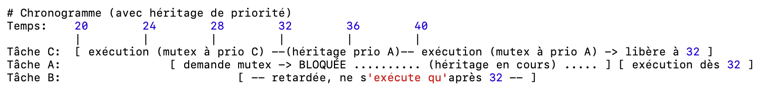
\includegraphics[width=15cm]{images/chrono2}
\end{figure}

Grâce à l’héritage, C (initialement prio 6) a fonctionné à un niveau de priorité 2 pendant qu’elle détenait le mutex réclamé par A. Ainsi, la tâche B (priorité 4) n’a jamais pu prendre le processeur tant que C n’avait pas fini sa section critique (achevée plus tôt, à t=32 dans notre exemple modifié). La tâche A a pu obtenir le mutex dès t=32, au lieu de t=36 ou plus dans le scénario sans héritage. Le temps d’attente de A a donc été réduit, et l’ordonnancement effectif respecte mieux la hiérarchie des priorités.

\pagebreak

\section{Analyse critique}
Le mécanisme d’héritage de priorité implémenté a permis de corriger l’inversion de priorité dans le cas étudié, mais il présente certaines limitations et repose sur des hypothèses simplificatrices. Tout d’abord, l’échange d’identités dans les files de priorité est une solution spécifique à cette implémentation qui suppose qu’une tâche n’hérite que d’une seule autre priorité à la fois. Si une tâche basse priorité C détient plusieurs mutex et bloque simultanément plusieurs tâches de priorités différentes, seul le plus prioritaire de ces tâches verra son niveau hérité par C (dans notre code, dès qu’une tâche plus prioritaire se présente, on ne gère pas d’héritage additionnel pour une seconde tâche). La gestion transitive de l’héritage (cas de chaînes où A bloque sur un mutex détenu par B qui lui-même attend un mutex détenu par C, etc.) n’est pas explicitement couverte par notre implémentation simplifiée.
\\\\
Ensuite, notre file d’attente de mutex est gérée en FIFO simple. Cela signifie qu’en l’absence d’héritage, l’ordre de réveil des tâches en attente n’est pas forcément optimal du point de vue de la priorité. Une amélioration possible serait d’utiliser une file à priorité pour les attentes de mutex : la tâche en attente la plus prioritaire serait réveillée en premier lors d’un m\_release, plutôt que strictement la première arrivée. Néanmoins, le protocole d’héritage de priorité atténue partiellement ce problème puisque la plus prioritaire aurait hérité du mutex plutôt que de rester en file.
\\\\
On peut également discuter du choix d’implémentation de l’héritage : nous avons opté pour une modification des structures de l’ordonnanceur (swap dans les files) plutôt que d’ajuster directement le champ priorite du TCB du propriétaire. Cette approche évite de parcourir toutes les tâches ou de réorganiser une file de manière complexe, au prix d’une certaine complexité conceptuelle. Une approche alternative aurait pu consister à augmenter tcb\_owner->priorite et à replacer la tâche propriétaire dans la file correspondant à sa nouvelle priorité ; cela aurait un effet similaire et peut être plus facile à tracer lors du débogage.
\\\\
Enfin, quelques hypothèses simplificatrices du mini-noyau limitent la portée de l’héritage de priorité : par exemple, on considère un nombre limité de niveaux de priorité (0–7) et un nombre maximal de tâches, ce qui facilite l’implémentation. Dans un système temps réel plus complet, il faudrait gérer des priorités sur une plage plus large et potentiellement dynamiques (besoin d’une structure de données plus performante qu’une simple boucle pour trouver la tâche suivante). De plus, des mécanismes tels que l’héritage de priorité transitive ou le protocole du plafond de priorité (priority ceiling) pourraient être envisagés pour traiter des scénarios complexes (plusieurs ressources imbriquées, évitement d’interblocages, etc.).

\pagebreak

\section{Conclusion et ouverture}

Ce mini-projet a permis d’implémenter un noyau temps réel minimaliste illustrant un ordonnanceur à priorité fixe avec la capacité de gérer des priorités dynamiques. L’étude du cas du mutex a mis en évidence le problème de l’inversion de priorité et montré qu’une solution simple d’héritage de priorité peut être intégrée afin de garantir le respect de l’ordonnancement préemptif par priorité.
\\\\
La solution apportée – bien qu’efficace dans les scénarios de base – gagnerait à être généralisée et renforcée pour un véritable système temps réel. En perspective, on peut envisager d’implémenter une gestion transitive complète de l’héritage de priorité afin de couvrir les cas de dépendances multiples, ainsi que d’autres protocoles de prévention de l’inversion de priorité comme le protocole du plafond de priorité, où chaque mutex possède un niveau de priorité maximal que ses utilisateurs peuvent hériter dès leur verrouillage pour éviter toute inversion. L’intégration de ces mécanismes plus avancés dépasse le cadre du mini-projet, mais le travail accompli fournit une base solide pour comprendre et aborder ces problématiques cruciales des systèmes temps réel embarqués.

\end{document}